\chapter{Future Work}\label{ch:future}

I have demonstrated in Chapter \ref{ch:paper} that our method works on a sample of previously studied stars, returning high-precision stellar parameters in-line with prior work \citep{Serenelli.Johnson.ea2017}. Our method is scalable to multiple input and output parameters, allowing for additional observational constraints to be easily added. In this chapter, I will briefly discuss a future extension to the method.

\section{Including an Asteroseismic Signature of Helium}

The effects of $\alpha_\mathrm{mlt}$ and $Y$ are more-or-less degenerate in the stellar observables. For example, for a star of a given age, mass and metallicity, increasing initial $Y$ or $\alpha_\mathrm{mlt}$ will increase its $T_\mathrm{eff}$. The effects of $\alpha_\mathrm{mlt}$ and $Y$ on typical stellar observables are also small, making it difficult for our models to distinguish between the two parameters. This manifests as an anti-correlation between the two parameters in our models. Therefore, if we improve our constraint on one, we will improve our inference of the other. Since $\alpha_\mathrm{mlt}$ is an approximation of convection and not a real physical quantity, we need an observable which relates closely to the helium abundance.

We should extend our model to include an independent measure of helium abundance in the star. Since helium lines are not present in the spectra of low-mass stellar atmospheres, we must look to other indicators of helium abundance. One such approach utilises asteroseismology. Stellar oscillations can provide a probe of rapid variation is stellar structure via a periodic signature in the p mode separations \citep[see e.g.][]{Broomhall.Miglio.ea2014}. This has been used to study the base of the convective zone \citep{Monteiro.Christensen-Dalsgaard.ea2000} and crucially, the boundary of the second helium (He \textsc{ii}) ionization zone \citep{Houdek.Gough2007}.

The boundary between the first and second helium ionization zones induces a peak in the adiabatic index (related to the sound-speed profile), noticeable in the convective regions of sufficiently cool, low-mass stars. This causes and acoustic glitch in the oscillation modes, $\nu$ -- a small deviation from the normal mode pattern in a star without He ionization. The amplitude of this glitch depends on the amount of helium present. This has been used with helioseismology to determine the helium enrichment near the solar surface \citep{Basu.Antia1995, Basu.Antia2004}. Recently, for example, the He \textsc{ii} glitch has been measured in samples of cool, low-mass stars \citep{Mazumdar.Monteiro.ea2014, Corsaro.DeRidder.ea2015, Verma.Raodeo.ea2017}. Inference of helium abundance can then either be made with comparison with stellar models or through asteroseismic inversion techniques \citep[e.g. for a the 16Cyg binary star system][]{Verma.Faria.ea2014, Buldgen.Salmon.ea2016}.

A recent study determining helium in a sample of low-mass dwarfs \citep{Verma.Raodeo.ea2019} characterises the small difference in $\nu$ due to the He \textsc{ii} ionization zone with the following equation based on the works of \citep{Houdek.Gough2007},
% \begin{equation}
%     \delta v_{\mathrm{He}}=A_{\mathrm{He}} v e^{-8 \pi^{2} \Delta_{\mathrm{He}}^{2} v^{2}} \sin \left(4 \pi \tau_{\mathrm{He}} v+\psi_{\mathrm{He}}\right),
% \end{equation}
\begin{equation}
    \delta v_{\mathrm{He}}=A_{\mathrm{He}}(\nu) \sin \left(4 \pi \tau_{\mathrm{He}} v+\psi_{\mathrm{He}}\right),
\end{equation}
% where $A_{\mathrm{He}}$ relates to the area beneath the peak in the adiabatic index, $\Delta_{\mathrm{He}}$ describes its width, $\tau_{\mathrm{He}$ is the acoustic depth of the boundary and . 
where $A_{\mathrm{He}}(\nu)$ is the amplitude of the glitch, $\tau_{\mathrm{He}}$ is the acoustic depth of the He \textsc{ii} zone and $\psi_{\mathrm{He}}$ is the phase term. The amplitude of the glitch depends on $\nu$, but \citet{Verma.Raodeo.ea2019} showed that an average amplitude across all observed frequencies, $\langle A_{\mathrm{He}} \rangle$, can be a good indicator of helium abundance.

Figure \ref{fig:glitch} shows an example of the glitch in KIC 10068307, a $\sim \SI{1.4}{\solarmass}$ dwarf star. We can see a small oscillating pattern in the echelle plot, particularly at low frequencies. The difference between the observed frequencies and the smoothed frequency pattern is also plot along with a fit from \citet{Verma.Raodeo.ea2017}. The component of the fit due to the He \textsc{ii} ionization zone can be used to extract $\langle A_{\mathrm{He}} \rangle$ for the star. 

\begin{figure}
    \begin{subfigure}[b]{0.5\linewidth}
        \centering
        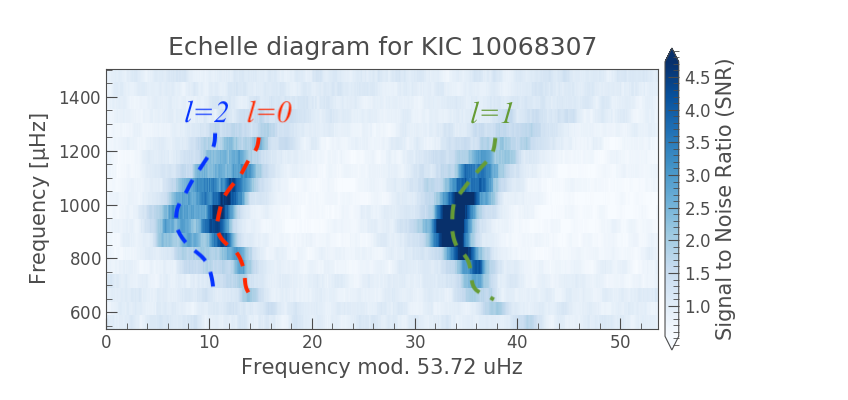
\includegraphics[trim={1cm 0 2.5cm 0},clip,width=\linewidth]{future/KIC10068307_echelle.png}
    \end{subfigure}%
    \begin{subfigure}[b]{0.5\linewidth}
        \centering
        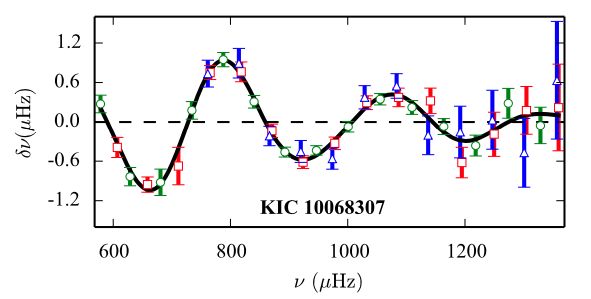
\includegraphics[width=\linewidth]{future/KIC10068307_glitch.png}
    \end{subfigure}
    \caption{\emph{Left}: an echelle diagram for a dwarf star (KIC 10068307) with the ridges according to each angular degree labelled. \emph{Right}: The small difference (glitch) in observed frequency $\nu$ compared with a smoothed frequency pattern for KIC 10068307 \citep{Verma.Raodeo.ea2017}.}
    \label{fig:glitch}
\end{figure}

In a future extension to the HBM method detailed in this report, I will include $\langle A_{\mathrm{He}} \rangle$ as a model output, determined from our models of stellar structure from MESA. Then, either using published values of the glitch amplitude available for the sample of low-mass dwarfs studied in this work \citep[e.g.][]{Verma.Raodeo.ea2017} or by performing my own analysis, I will introduce it as a new observable quantity. This also gives us potential to hierarchically model the surface helium abundance. Once we can improve constraints on helium, we will improve the modelling of $\alpha_\mathrm{mlt}$. This will lead to testing other ways of pooling $\alpha_\mathrm{mlt}$ as a function of stellar properties.

% \section{Higher Masses and Evolved Stars}

% Our next step is to include intermediate-mass stars with masses from approx. 1.2 solar masses to 3.0 solar masses.
